\chapter{Implementation}
\label{implementation}

\section{ZeroMQ Protocols}

For a quick background on ZeroMQ socket types and message patterns, please see Appendix \ref{zeromq_primer}.

\subsection{Topology Protocol}
\label{proto_topo}

The \dcamp distributed topology is dynamically established as the Root node sends out its discovery message and receives
join messages from Base nodes. Once a Base node responds to the Root, the Base node is given its assignment.
Additionally, the Root node can shutdown the system using this same protocol but responding with a "stop" message
instead of an assignment.

\begin{figure}[H]
\vspace{+10pt}
\begin{verbatim}
topo-discovery = *discover join
discover       = R-MARCO
join           = B-POLO ( R-ASSIGN / R-STOP / R-WTF )
\end{verbatim}
\vspace{-5pt}
\caption[Topology Protocol]
        {Topology Protocol: \texttt{R-} represents the Root node sending a message and \texttt{B-}
         represents a Base node sending a message.}
\label{fig:proto_topo_spec}
\end{figure}

\begin{figure}[H]
    \centering
    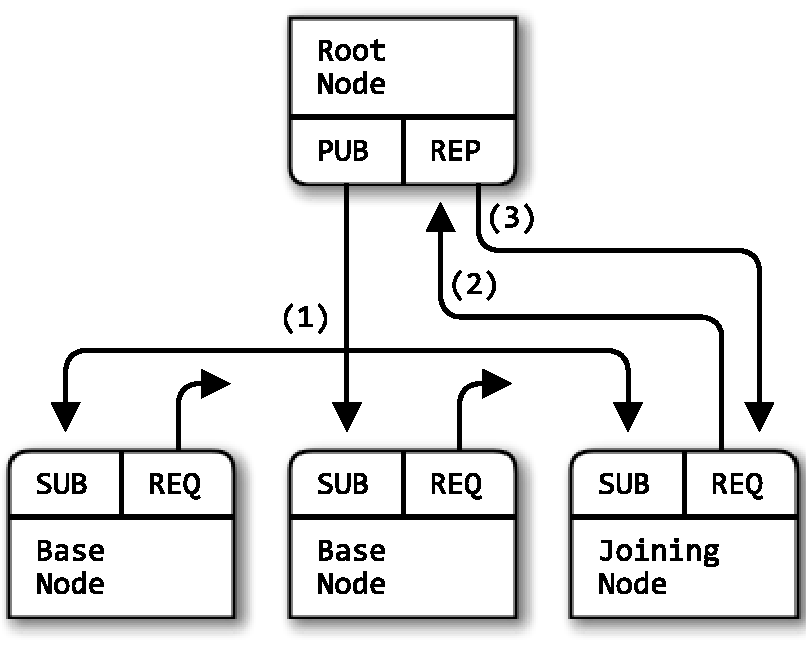
\includegraphics[scale=0.5]{topo.pdf}
    \label{fig:proto_topo_image}
    \caption{Topology Protocol Diagram}
\end{figure}

\subsubsection{Message Definitions}

\textbf{\texttt{TOPO}} is a generic topology message consisting of four frames. This message type is designed to be sent
across a PUB/SUB connection, from which subscribers filter incoming messages using the first frame. This design proves
useful for the \hyperref[proto_reco]{Recovery Protocols}.

The \texttt{MARCO} message is simply shorthand for \texttt{TOPO(key="/MARCO")}.

\begin{figure}[H]
\vspace{+10pt}
\begin{verbatim}
Frame 0: key, as 0MQ string
Frame 1: root address, as 0MQ string
Frame 2: root UUID, 16 bytes in network order
Frame 3: <empty> or content, as 0MQ string
\end{verbatim}
\vspace{-20pt}
\caption{\texttt{TOPO} Message Definition}
\label{fig:message_topo}
\end{figure}

\textbf{\texttt{CONTROL}} is a generic control message consisting of four frames and designed to be sent across a
REQ/REP connection. The \texttt{POLO}, \texttt{ASSIGN}, and \texttt{STOP} messages are shorthand for
\texttt{CONTROL(command="POLO")}, \texttt{CONTROL(command="ASSIGN")}, and \texttt{CONTROL(command="STOP")} respectively.

In the case of \texttt{ASSIGN}, the third frame contains the specific topology instructions (level-one collector, leaf
node, etc.) being sent to the Base node.

\begin{figure}[H]
\vspace{+10pt}
\begin{verbatim}
Frame 0: command, as 0MQ string
Frame 1: base address, as 0MQ string
Frame 2: base UUID, 16 bytes in network order
Frame 3: properties, JSON-encoded, as 0MQ string

command     = "polo" / "assignment"
properties  = *( parent / level / group )
parent      = "parent=" <node-address>
level       = "level=" ( "root" / "branch" / "leaf" )
group       = "group=" <group-identity>
\end{verbatim}
\vspace{-20pt}
\caption{\texttt{CONTROL} Message Definition}
\label{fig:message_control}
\end{figure}

\textbf{\texttt{WTF}} is \dcamp's error message type. It has three frames (though Frame 2 may be empty) with the first
designed to make error detection simple.

\begin{figure}[H]
\vspace{+10pt}
\begin{verbatim}
Frame 0: "WTF", as 0MQ string
Frame 1: error code, 4 bytes in network order
Frame 2: <empty> or error message, as 0MQ string
\end{verbatim}
\vspace{-20pt}
\caption{\texttt{WTF} Message Definition}
\label{fig:message_wtf}
\end{figure}

\subsection{Configuration Replication Protocol}
\label{proto_config}

\dcamp configuration and topology state are replicated across the system using key-value pairs, with the keys laid out
in a hierarchical fashion. This lends itself nicely to PUB/SUB topic filtering.

For example, because a Metric node only needs the configuration values for its particular group, the node subscribes
only to the \texttt{"/CONFIG/<group-name>/"} topic. Any \texttt{KVPUB} whose key does not start with this string is
then discarded.

In practice, Metric nodes need more than just their group-specific configuration, but the general principle holds true:
nodes only receive the configuration data they require and nothing more. In the case of first-level Collector nodes, they
receive all updates since they are fail-over candidates for the root node.

\begin{figure}[H]
\vspace{+10pt}
\begin{verbatim}
config-replication = *update / snap-sync
update             = P-KVPUB / P-HUGZ
snap-sync          = C-ICANHAZ ( ( *P-KVSYNC P-KTHXBAI ) / P-WTF )
\end{verbatim}
\vspace{-5pt}
\caption[Configuration Protocol Specification]
	{Configuration Protocol Specification: \texttt{P-} represents the parent node (Root or Collector) sending a
	 message and \texttt{C-} represents the child node sending a message.}
\label{fig:proto_config_spec}
\end{figure}

A newly assigned first-level Collector node will first subscribe to new configuration updates from the Root node and
then send a configuration snapshot request to the Root node. A newly assigned Sensor (or non-first-level Collector) node
will first subscribe to new configuration updates from its parent Collector node, and then send its parent Collector
node a filtered configuration snapshot request. Once its snapshot has been successfully received, a node will process
any pending configuration updates and then, in the case of a Collector node, respond to child node snapshot requests.

The \dcamp configuration replication algorithm adheres to the Clustered Hashmap Protocol\cite{chp} with a few minor
(and one major) modifications:

\begin{enumerate}
\item only the Root node may write updates to the configuration,
\item the full configuration table will be replicated across all first-level Collector nodes (lower-level nodes may
      filter their configuration to only store relevant data),
\item a different set of command names are used (as described below), and
\item configuration updates are distributed via the \dcamp hierarchy (instead of directly from the Root node).
\end{enumerate}

\begin{figure}[H]
    \centering
    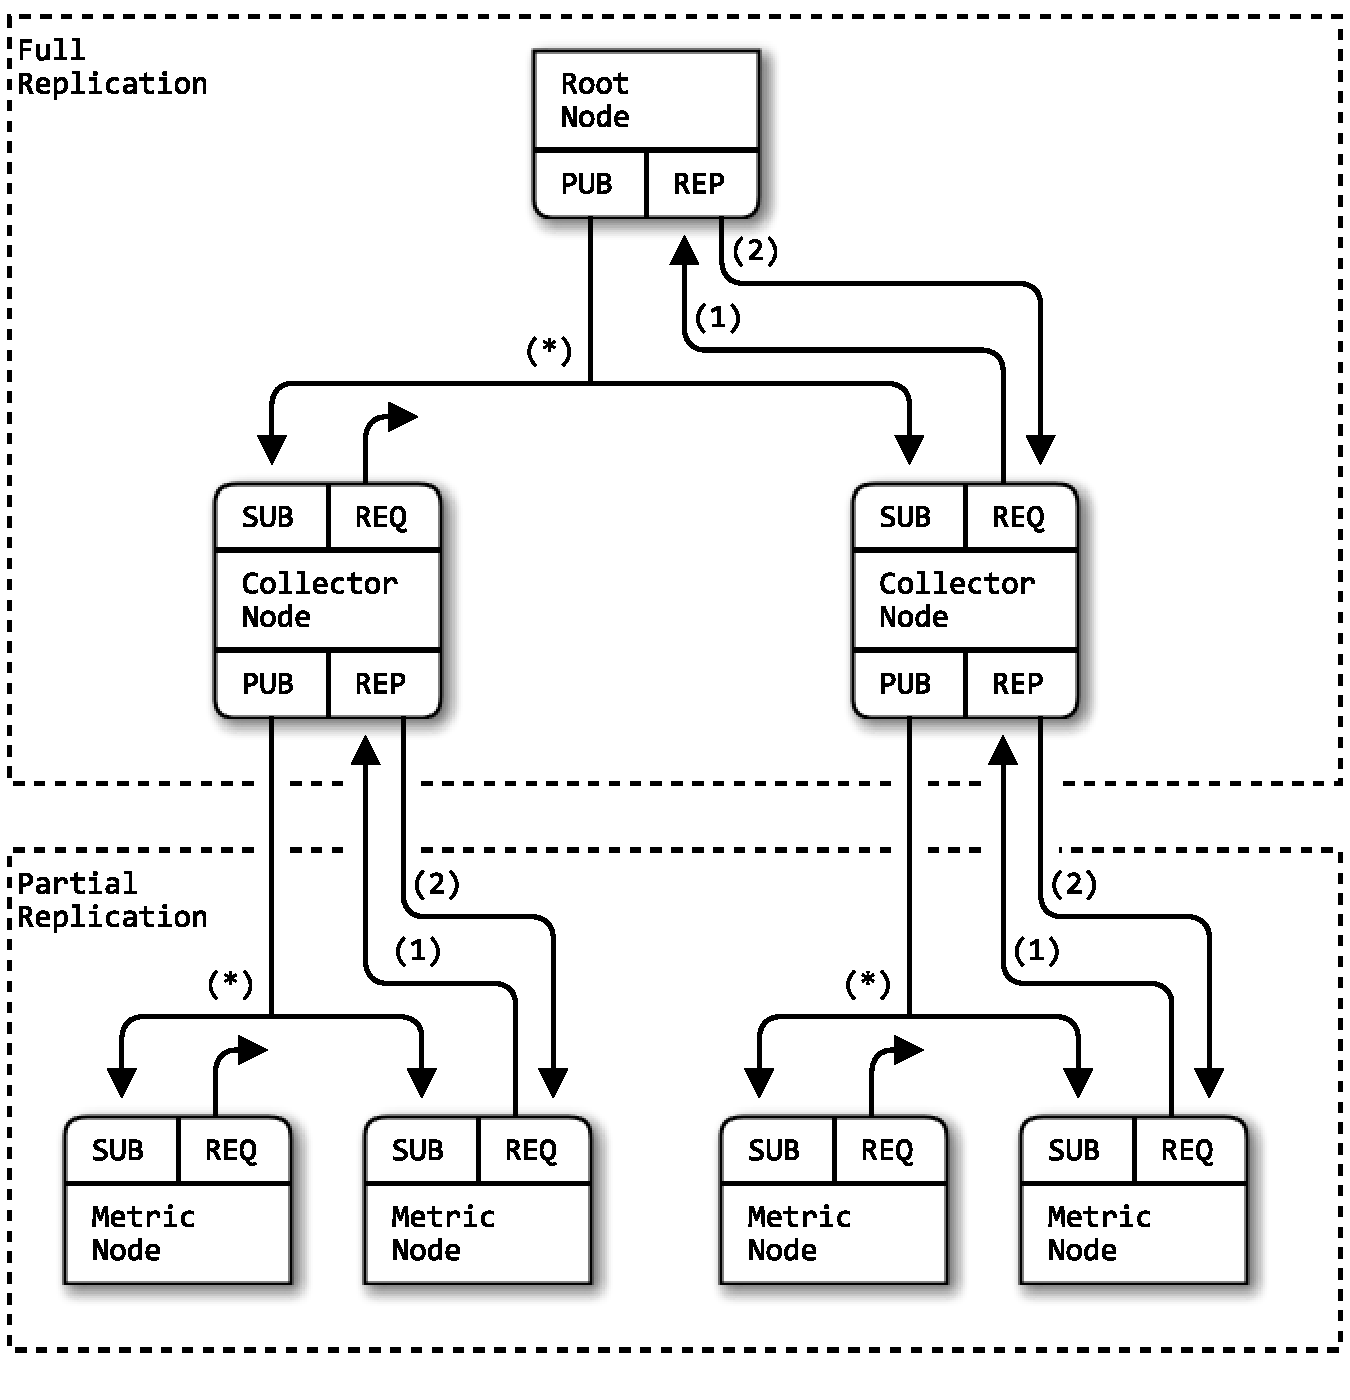
\includegraphics[scale=0.5]{config.pdf}
    \caption{Configuration Protocol Diagram}
    \label{fig:proto_config_image}
\end{figure}

\subsubsection{Message Definitions}

These messages come from the CHP protocol. Additionally, a \texttt{WTF} error message may be sent by the parent in case
of error. It should be noted, each of the following messages is really the same five-frame format with varying keys and
semantics.

As shown in Figure \ref{fig:proto_config_spec}, the \texttt{ICANHAZ}, \texttt{KVSYNC}, and \texttt{KTHXBAI} messages are
sent across a REQ/REP connection type. \texttt{KVPUB} (as the name would imply) along with the \texttt{HUGZ} heartbeat
message are designed for the PUB/SUB pattern.

\textbf{\texttt{ICANHAZ}} is a configuration snapshot request sent by the child node when it first starts. Multiple
\texttt{ICANHAZ} requests can be sent for the different topics or subtrees needed by the node, and the node will not
begin normal operation until all of the requested values have been received.

\begin{figure}[H]
\vspace{+10pt}
\begin{verbatim}
Frame 0: "ICANHAZ", as 0MQ string
Frame 1: <empty>
Frame 2: <empty>
Frame 3: <empty>
Frame 4: subtree specification, as 0MQ string
\end{verbatim}
\vspace{-20pt}
\caption{\texttt{ICANHAZ} Message Definition}
\label{fig:message_icanhaz}
\end{figure}

\textbf{\texttt{KVSYNC}} is a configuration snapshot response message. For every key-value pair within the requested
subtree, a \texttt{KVSYNC} message is sent to the child node. Note: if no values exist for a requested subtree, a
\texttt{KTHXBAI} message will be the only response received by the child node.

The sequence number in Frame 1 SHOULD be ignored by the recipient since no order guarantees exist for configuration
snapshots requests.

\begin{figure}[H]
\vspace{+10pt}
\begin{verbatim}
Frame 0: key, as 0MQ string
Frame 1: sequence number, 8 bytes in network order
Frame 2: <empty>
Frame 3: <empty>
Frame 4: value, as blob
\end{verbatim}
\vspace{-20pt}
\caption{\texttt{KVSYNC} Message Definition}
\label{fig:message_kvsync}
\end{figure}

\textbf{\texttt{KTHXBAI}} marks the end of a successful snapshot request. Frame 4 MUST contain the highest sequence
number of all the values in the configuration snapshot.

\begin{figure}[H]
\vspace{+10pt}
\begin{verbatim}
Frame 0: "KTHXBAI", as 0MQ string
Frame 1: sequence number, 8 bytes in network order
Frame 2: <empty>
Frame 3: <empty>
Frame 4: subtree specification, as 0MQ string
\end{verbatim}
\vspace{-20pt}
\caption{\texttt{KTHXBAI} Message Definition}
\label{fig:message_kthxbai}
\end{figure}

\textbf{\texttt{KVPUB}} is a configuration update sent from parent to child. The sequence number in Frame 1 must be
monotonically increasing. When a \texttt{KVPUB} is received which has a sequence number lower than a previously received
\texttt{KVPUB}, the node MUST delete its saved configuration values and request a new snapshot.

Frame 2 SHOULD contain the UUID of the node from which the value originated. In \dcamp, this should only be the Root
node's UUID. Frame 3 MAY contain additional properties for the key-value pair, such as an ephemeral time-to-live.

\begin{figure}[H]
\vspace{+10pt}
\begin{verbatim}
Frame 0: key, as 0MQ string
Frame 1: sequence number, 8 bytes in network order
Frame 2: UUID, 16 bytes in network order
Frame 3: properties, JSON-encoded, as 0MQ string
Frame 4: value, as blob
\end{verbatim}
\vspace{-20pt}
\caption{\texttt{KVPUB} Message Definition}
\label{fig:message_kvpub}
\end{figure}

\textbf{\texttt{HUGZ}} is the heartbeat message sent from parent to child when the rate of \texttt{KVPUB} messages being
sent drops below a predetermined threshold. The \texttt{HUGZ} message is critical to maintaining topological consistency
in \dcamp.

\begin{figure}[H]
\vspace{+10pt}
\begin{verbatim}
Frame 0: "HUGZ"
Frame 1: 00000000
Frame 2: <empty>
Frame 3: <empty>
Frame 4: <empty>
\end{verbatim}
\vspace{-20pt}
\caption{\texttt{HUGZ} Message Definition}
\label{fig:message_hugz}
\end{figure}

\subsection{Data Flow Protocol}
\label{proto_data}

There are two data flow protocols in the \dcamp system: the external protocol for data flowing from one node to the next
(via PUB/SUB) and the internal protocol for data flowing between components of a single node (via PUSH/PULL). Both
protocols have the same specification and use the same message formats.

\begin{figure}[H]
    \centering
    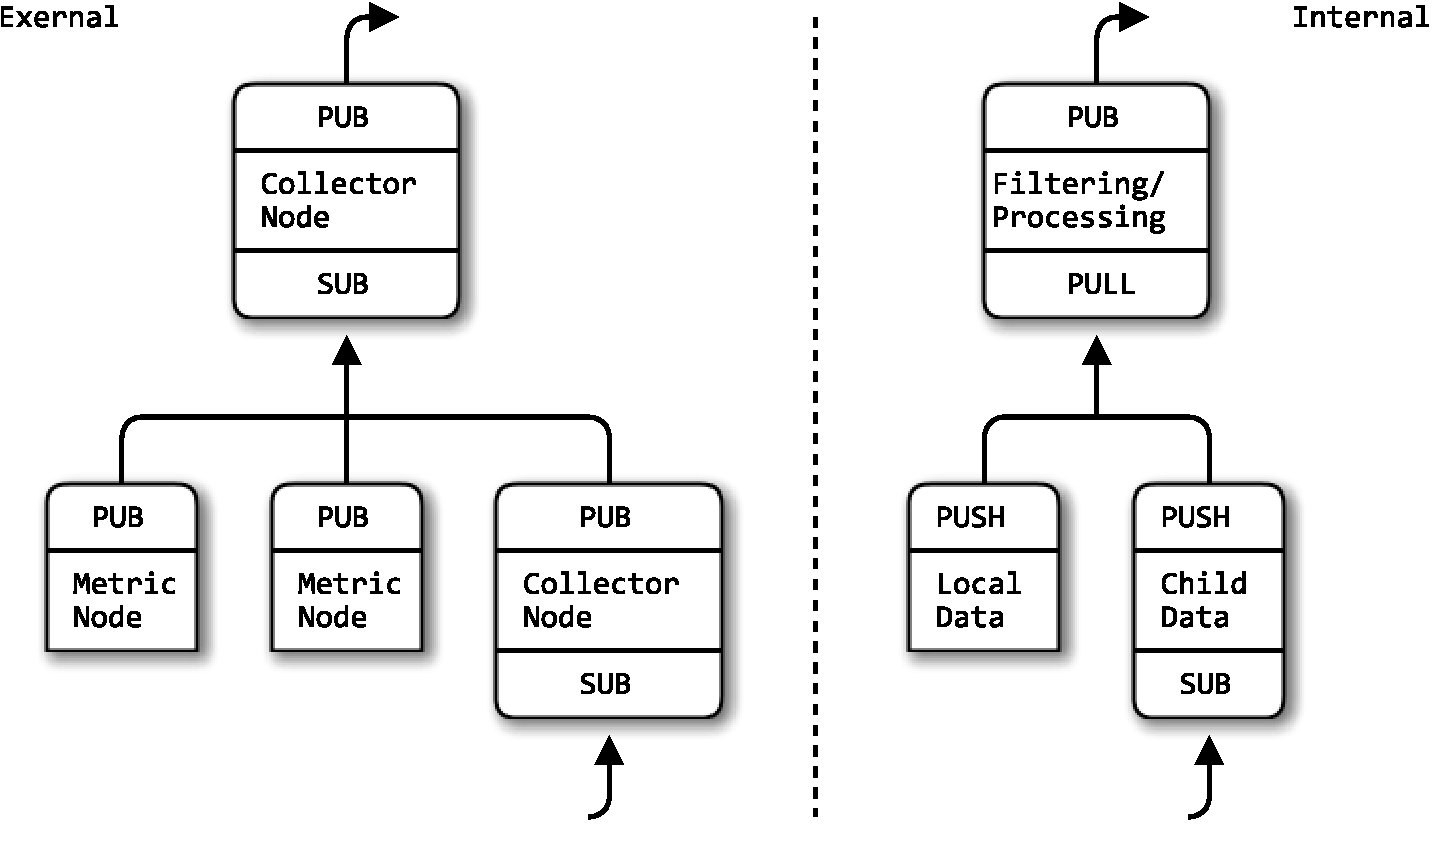
\includegraphics[scale=0.5]{data.pdf}
    \caption{Data Flow Diagram}
    \label{fig:proto_data_image}
\end{figure}

The \dcamp data flow protocol is very simple, comprised of a single data message type. The data flows from one node to
another via PUB/SUB sockets. Internally, data flows from the upstream data producers, through a filtering/processing
unit, and out to downstream data consumers via PUSH/PULL sockets.

When data rate is slower than a predefined threshold, heartbeats are sent instead to keep inter-node connections alive.

\begin{figure}[H]
\vspace{+10pt}
\begin{verbatim}
data-flow = *( METRIC / HUGZ )
\end{verbatim}
\vspace{-5pt}
\caption[Data Flow Specification]
	{Data Flow Specification: All messages are sent from child (Metric or Collector) to parent (Collector or Root).}
\label{fig:proto_data_spec}
\end{figure}

\subsubsection{Performance Measurement}

When discussing performance measurement, it is important to understand how metrics are sampled, calculated, and
presented to an end user.

Performance metrics, also called counters, are usually monotonically increasing values. That is, reading its raw,
instantaneous value is virtually meaningless; to correctly read the counter it must be sampled at two different points
in time and then calculated.

For example, when displaying a graph of data point for non-basic metric types, each data point is really a calculated
value of the value at the current timestamp and that at the previous timestamp. It is possible to look at fewer data
samples to first get a course-grain view (e.g. five-minute samples) of the metric before drilling in a looking at
finer-grain samples (e.g. one-second samples).

Non-monotonically increasing counters do exist (e.g. disk speed, Ethernet uplink speed, etc.), but these are usually
fairly static configuration values and do not need to be sampled frequently. \dcamp supports these types of counters
with the ``basic'' metric type.

Table \ref{tab:metric_types} shows how each of the \dcamp metric types are calculated. Note: unlike some other
performance measurement frameworks\cite{ganglia}, \dcamp stores all metrics in their raw, uncalculated form and only
presents a calculated value upon display.

\renewcommand{\arraystretch}{1.5}
\begin{table}
\begin{tabular}{ l|l|l }
\hline
\textbf{Type} & \textbf{Contents of Single Sample} & \textbf{Calculation of Two Samples}
\tabularnewline
\hline
basic & raw value at specified timestamp & \( C = V_{t_2} \)
\tabularnewline
delta & raw value at specified timestamp & \( C = V_{t_2} - V_{t_1} \)
\tabularnewline
rate & raw value at timestamp & \( C = \frac{V_{t_2} - V_{t_1}}{t_2 - t_1} \)
\tabularnewline
average & raw value and base value at timestamp & \( C = \frac{V_{t_2} - V_{t_1}}{B_{t_2} - B_{t_1}} \)
\tabularnewline
percent & raw value and base value at timestamp & \( C = 100 \frac{V_{t_2} - V_{t_1}}{B_{t_2} - B_{t_1}} \)
\tabularnewline
\end{tabular}
\caption[Metric Types]
        {Metric Types: \(C\) represents the value calculated from two samples taken at \(t_1\) and \(t_2\). \(V\) is the
	 value and \(B\) is the base value in the \texttt{METRIC} message}
\label{tab:metric_types}
\end{table}

\subsubsection{Message Definitions}

\textbf{\texttt{METRIC}} is a five-frame message containing the performance metric data sampled by the Sensor service or
calculated by the Aggregation service. The \texttt{HUGZ} message is simply shorthand for \texttt{METRIC(type="HUGZ")}.

A single data sample MUST contain: source identifier (node or aggregation), metric identifier, timestamp, and one or two
values depending on the metric type.

In case of \texttt{HUGZ}, no other property strings are used, and Frames 3 through 5 are all empty. Frame 4 will be
non-empty for average and percent types.

NOTE: This message needs to be cleaned up...its a bit too verbose. I think just the config-seqid is needed to identify
      the metric being sampled.

\begin{figure}[H]
\vspace{+10pt}
\begin{verbatim}
Frame 0: data source (leaf or collector node address), as 0MQ string
Frame 1: properties, JSON-encoded as 0MQ string
Frame 2: time in ms epoch utc, 8 bytes in network order
Frame 3: value, 8 bytes in network order
Frame 4: base value, 8 bytes in network order; only for average and percent types

properties = *( type / detail / config / seqid )
type       = "type=" ( "HUGZ" / "basic" / "delta" / "rate" / "average" / "percent" )
detail     = "detail=" <string>
config     = "config-name=" <string>
seqid      = "config-seqid=" <integer>
\end{verbatim}
\vspace{-20pt}
\caption{\texttt{METRIC} Message Definition}
\label{fig:message_metric}
\end{figure}

\subsection{Recovery Protocols}
\label{proto_reco}

The \dcamp Recovery Protocols are used for the \hyperref[algor_promo]{Promotion} and \hyperref[algor_elect]{Election}
algorithms and use the same base messages as the \hyperref[proto_topo]{Topology Protocol}, \texttt{TOPO} and
\texttt{CONTROL}.

\begin{figure}[H]
\vspace{+10pt}
\begin{verbatim}
branch-recovery  = *sos group-stop
sos              = M-SOS R-KEEPCALM
group-stop       = R-GROUP M-POLO R-STOP
\end{verbatim}
\vspace{-5pt}
\caption[Branch Recovery Protocol]
	{Branch Recovery Protocol: \texttt{R-} represents the \textit{Root} node sending a message and \texttt{M-}
	 represents a \textit{Metric} node sending a message.}
\label{fig:proto_reco_branch_spec}
\end{figure}

The Branch Recovery Protocol is initiated by \textit{Metric} nodes when they detect their \textit{Collector} has died.
Once the \textit{Root} node has received an \texttt{SOS} message from at least one third of the branch's \textit{Metric}
nodes, the \textit{Root} proceeds to shutdown the entire branch using the ``stop'' Topology Protocol. Once shut down, a
new \textit{Collector} is selected and the branch is rebuilt using the standard ``discover'' Topology Protocol.

\begin{figure}[H]
    \centering
    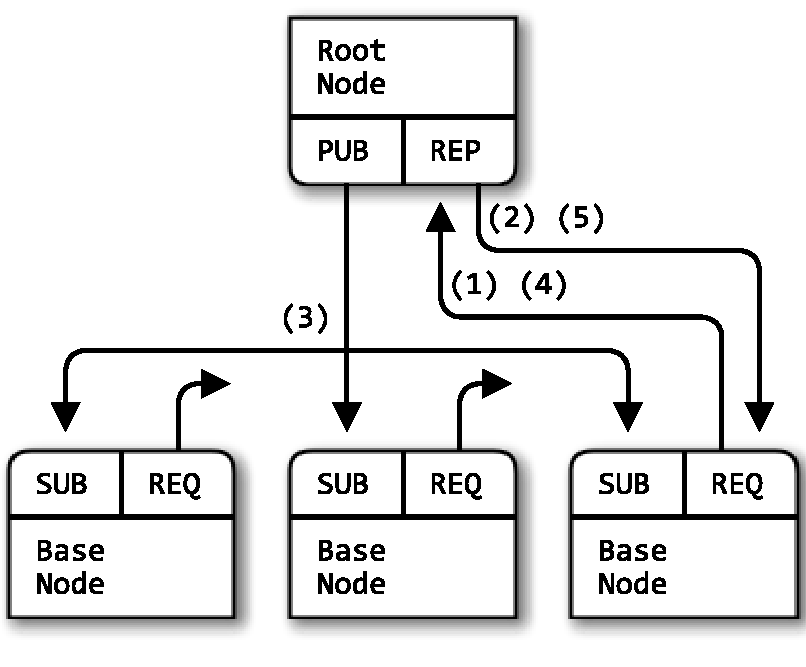
\includegraphics[scale=0.5]{branch-recovery.pdf}
    \label{fig:proto_branch_reco_image}
    \caption[Branch Recovery Protocol Diagram]
	    {Branch Recovery Protocol Diagram: (1) \textit{Metric} nodes send \texttt{SOS} requests, (2) \textit{Root}
	     replies with \texttt{KEEPCALM}, (3) \textit{Root} sends \texttt{GROUP} only to nodes in branch, (4)
	     \textit{Metric} nodes send \texttt{POLO} requests, (5) \textit{Root} replies with \texttt{STOP}}
\end{figure}

\texttt{SOS} and \texttt{KEEPCALM} are shorthand for the \texttt{CONTROL} message with a command value of \texttt{"sos"}
and \texttt{"keepcalm"} respectively. The \texttt{POLO} and \texttt{STOP} messages come directly from the Topology
Protocol.

The \texttt{GROUP} message is similarly shorthand for the \texttt{TOPO} message with a key value of
\texttt{"/GROUP/<group-name>"}. This takes advantage of ZeroMQ's Pub-Sub filtering to only stop the faulty branch.

\begin{figure}[H]
\vspace{+10pt}
\begin{verbatim}
root-recovery  = *election
election       = C-WUTUP *C-YO C-IWIN
\end{verbatim}
\vspace{-5pt}
\caption[Root Recovery Protocol]
        {Root Recovery Protocol: \texttt{C-} represents a \textit{Collector} node sending a message.}
\label{fig:proto_reco_root_spec}
\end{figure}

As each \textit{Collector} node detects the \textit{Root} node has died, it attempts to start an election via the
\texttt{WUTUP} message. \textit{Collector} nodes with higher UUIDs will respond to the first \textit{Collector} by
sending the \texttt{YO} message. If no \texttt{YO} messages are received by the first \textit{Collector}, the
\texttt{IWIN} message is sent out to all \textit{Collector} nodes, self-declaring the first \textit{Collector} as the
new Root.

\begin{figure}[H]
    \centering
    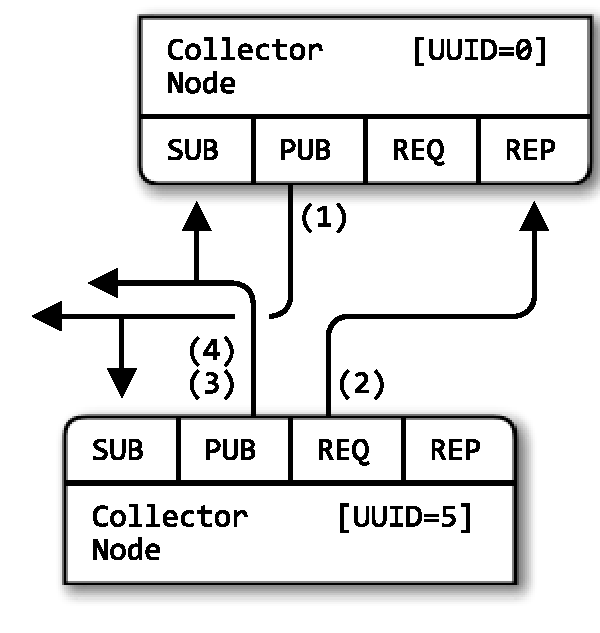
\includegraphics[scale=0.5]{root-recovery.pdf}
    \label{fig:proto_root_reco_image}
    \caption[Root Recovery Protocol Diagram]
	    {Root Recovery Protocol Diagram: (1) \texttt{WUTUP}, (2) \texttt{YO}, (3) \texttt{WUTUP}, (4) \texttt{IWIN}}
\end{figure}

The \texttt{WUTUP} and \texttt{IWIN} messages are shorthand for \texttt{TOPO(key="/RECOVERY/wutup"} and
\texttt{TOPO(key="/RECOVERY/iwin"} respectively. The \texttt{YO} message is shorthand for
\texttt{CONTROL(command="yo")}.


\section{Configuration}

\subsection{Node Specification}

Nodes may be specified individually (DNS-resolvable name or IP Address) or as groups (IP subnet). Additionally, nodes
may be included or excluded based on DNS name or IP Address matching. Name matching does a case-insensitive comparison
of the node's DNS name; left, right, or whole name matching can be specified. Address matching checks that the node's IP
Address falls within a given subnet (i.e. IP Address and mask length).

\begin{figure}[ht]
    \begin{lstlisting}
    node-spec        = node / node-group
    node             = address ":" port
    address          = hostname / ip-address
    node-group       = group-name 1*( node / subnet ) *filter
    subnet           = ip-address "/" mask-length
    filter           = [ "+" / "-" ] ( hostname-match / subnet-match )
    hostname-match   = [ ( "L" / "R" / "W" ) SP ] partial-hostname
    subnet-match     = subnet
    \end{lstlisting}
    \caption{Configuration File - Node Specification}
    \label{fig:config_file_node}
\end{figure}

\subsection{Sample Specification}

Performance metric samples are specified as:

\begin{enumerate}
\item the node(s) on which to sample the data,
\item the rate at which data should be sampled,
\item the threshold past which data should be reported, and lastly
\item the actual performance metric to be sampled.
\end{enumerate}

The report threshold can be specified as "hold and report every N seconds" or "report when the metric value is
greater/less than X". When "hold" is specified (via an *), all metric values sampled during the time limit are sent.

\begin{figure}[ht]
    \begin{lstlisting}
    sample-spec      = 1*sample
    sample           = sample-rate [ report-threshold ] metric
    sample-rate      = 1*DIGIT "s" ; seconds
    report-threshold = ( "*" 1*DIGIT "s" ) / ( ( "<" / ">" ) 1*DIGIT ) ; seconds or raw value
    metric           = "CPU" / "DISK" / "NETWORK"
    \end{lstlisting}
    \caption{Configuration File - Sample Specification}
    \label{fig:config_file_sample}
\end{figure}

NOTE ABOUT ACCUMULATION (DOESN'T WORK)

\begin{itemize}
\item filtering could be done two ways: accumulatively and discretely.
\item accumulative means we send only one final value for each time range (e.g. collect every second but report every
      minute, so 60 samples are combined into a single value and sent)
\item discrete means we send each constituent value for each time range, but they are "held" until the time limit is
      reached
\item how do these two filtering methods interact with value-based limits? are they always discrete?
\item ACTUALLY: accumulation is not valuable for monotonically increasing values--it is the same as just sampling at the
      slower frequency. accumulation is only valuable for non-monotonically increasing values. but in that case, one
      should find the raw, monotonically increasing values from which it is calculated.
\end{itemize}

